% !TEX root = IBL-InsolvabilityOfQuintic.tex
\chapter{Galois Theory}
\label{chapter:GaloisTheory}
\thispagestyle{empty}

We finished Chapter~\ref{chapter:AlgebraicExtensions} by computing automorphism groups of field extensions. We also began to connect the subfields of an extension  field $L$ of $F$ to subgroups of $\Aut(L/F)$.  We  now narrow our focus on which types of extension fields we consider, and in doing so, we significantly sharpen what we can say about this connection. It will be lynchpin of our argument showing that not all polynomials over $\mathbb{Q}$ are solvable by radicals over $\mathbb{Q}$.

Also, from here on, we will exclusively focus on subfields of $\mathbb{C}$. This will streamline (and simplify) our work, but it will also slightly obscure the general theory. Which is to say, this is more the beginning of the story than the end. 

% % % % % % % % % % % % % % % % % % % % % % % % % % % % % % % % % % % % % % % % % % % %
% % % % % % % % % % % % % % % % % % % % % % % % % % % % % % % % % % % % % % % % % % % %
% SECTION
% % % % % % % % % % % % % % % % % % % % % % % % % % % % % % % % % % % % % % % % % % % %
% % % % % % % % % % % % % % % % % % % % % % % % % % % % % % % % % % % % % % % % % % % %
\section{Galois extensions and Galois groups}

\begin{definition}\label{def.SplittingField}
Let $F$ be a subfield of $\mathbb{C}$, and let $p(x) \in F[x]$. Define $F^{p(x)}$ to be the subfield of $\mathbb{C}$ generated by $F$ and all roots of $p(x)$; thus,  $F^{p(x)}=F(r_1,\ldots,r_n)$ where $r_1,\ldots,r_n$ are all of the roots of $p(x)$ in $\mathbb{C}$.
\end{definition}

For example, if  $p(x) = x^5 - 1$, then by Theorem~\ref{thm.nthRoots1}, the roots of $p(x)$ are $1,\zeta_5,\zeta_5^2,\zeta_5^3,\zeta_5^4$, so $\mathbb{Q}^{p(x)}=\mathbb{Q}(1,\zeta_5,\zeta_5^2,\zeta_5^3,\zeta_5^4)$.

\begin{problem}\label{prob.QAdjoinZeta5IsGalois}
Let $p(x) = x^5 - 1$. Use Theorem~\ref{thm.FieldAdjoinElementsContainedInField} to explain why $\mathbb{Q}^{p(x)}=\mathbb{Q}(\zeta_5)$.
\end{problem}

\begin{problem}\label{prob.QAdjoinCubeRoot2IsNotASplittingField}
Let $p(x) = x^3 - 2$. Explain why $\mathbb{Q}^{p(x)}\neq\mathbb{Q}(\sqrt[3]{2})$.
\end{problem}

\begin{problem}\label{prob.ShowFieldIsASplittingField}
For each field $F$ below, find a polynomial $p(x)\in \mathbb{Q}[x]$ such that $F=\mathbb{Q}^{p(x)}$.
\begin{multicols}{2}
\begin{enumerate}
\item $F=\mathbb{Q}(\sqrt{2})$
\item $F=\mathbb{Q}(\sqrt{2},i)$
\item $F=\mathbb{Q}(\sqrt[3]{2},\zeta_3)$
\item $F=\mathbb{Q}(\zeta_{12})$
\end{enumerate}
\end{multicols}
\end{problem}

\begin{definition}
Let $F\subseteq K$ be subfields of $\mathbb{C}$.
\begin{enumerate}
\item We say that $K$ is a \textbf{Galois extension} of $F$ if $K = F^{p(x)}$ for some $p(x) \in F[x]$.
\item If $K$ is a Galois extension of $F$, then $\Aut(K/F)$ is called the \textbf{Galois group} of $K$ over $F$.
\end{enumerate}
\end{definition}

Revisiting Problem~\ref{prob.ShowFieldIsASplittingField} with this new terminology, we see that each of $\mathbb{Q}(\sqrt{2})$, $\mathbb{Q}(\sqrt{2},i)$, $\mathbb{Q}(\sqrt[3]{2},\zeta_3)$, and $\mathbb{Q}(\zeta_{12})$ are Galois extensions of $\mathbb{Q}$. Also, Problem~\ref{prob.QAdjoinCubeRoot2IsNotASplittingField} hints at the fact that $\mathbb{Q}(\sqrt[3]{2})$ might not be a Galois extension of $\mathbb{Q}$ (but there is more to prove to establish that).

Let's generalize parts of Problem~\ref{prob.ShowFieldIsASplittingField} and record some types of extensions that are always Galois.

\begin{theorem}\label{QAdjoinSquareRootIsGalois}
Let $a\in \mathbb{Q}$. Then $\mathbb{Q}(\sqrt{a})$ is a Galois extension of $\mathbb{Q}$.
\end{theorem}

\begin{theorem}\label{QAdjoinZetanIsGalois}
Let $n$ be a positive integer. Then $\mathbb{Q}(\zeta_{n})$ is a Galois extension of $\mathbb{Q}$.
\end{theorem}

As mentioned above, $\mathbb{Q}(\sqrt[3]{2})$ might not be a Galois extension of $\mathbb{Q}$, but it is true that  $F(\sqrt[3]{2})$ a Galois extension of $F$ provided $F$ contains $\zeta_3$. The next theorem addresses this.

\begin{theorem}\label{QAdjoinRadicalIsGaloisOverFieldWithRootsUnity}
Let $F$ be a subfield of $\mathbb{C}$. Suppose that $r\in \mathbb{C}$ and $r^n\in F$ for some positive integer $n$. If $\zeta_n\in F$, then $F(r)$ is a Galois extension of $F$.
\end{theorem}

% % % % % % % % % % % % % % % % % % % % % % % % % % % % % % % % % % % % % % % % % % % %
% SUBSECTION
% % % % % % % % % % % % % % % % % % % % % % % % % % % % % % % % % % % % % % % % % % % %
\subsection{Size of Galois groups}
The next fact highlights the importance of Galois extensions. The point is roughly that the automorphism group of a Galois extension has the ``expected'' number of automorphisms; whereas, automorphism groups of non-Galois extension will necessarily have fewer.

\begin{fact}\label{fact.SizeGaloisGroup}
Let $F$ be a subfield of $\mathbb{C}$. If $K$ is a Galois extension of $F$, then $|\Aut(K/F)| = [K:F]$.
\end{fact}

Fact~\ref{fact.SizeGaloisGroup} is extremely powerful. Let's start by seeing how it can help streamline the computation of certain automorphism groups.

\begin{problem}\label{prob.AutQAdjoinCubeRoot2AndZeta3OverQ}
Let $L = \mathbb{Q}(\sqrt[3]{2},\zeta_3)$. Let's determine $\Aut(L/\mathbb{Q})$. Recall from Problem~\ref{prob.ShowFieldIsASplittingField} that $L$ is a Galois extension of $\mathbb{Q}$.  
\begin{enumerate}
\item What is minimal polynomial for $\sqrt[3]{2}$ over $\mathbb{Q}$? Why?
\item What is minimal polynomial for $\zeta_3$ over $\mathbb{Q}(\sqrt[3]{2})$? Why?
\item Use Theorem~\ref{thm.BasisChainExtensionField} to explain why $[L : \mathbb{Q}] = 6$.
\item Let $\phi\in  \Aut(\mathbb{Q}(\sqrt[3]{2},\zeta_3)/\mathbb{Q})$. Use Theorem~\ref{thm.HomFixingFPermutesRootsOfPolysOverF} to explain why there are only 3 choices for $\phi(\sqrt[3]{2})$ and only two choices for $\zeta_3$. What are they?
\item Complete the table of possible elements of $\Aut(L/\mathbb{Q})$.
\begin{center}
\tabulinesep = 2mm
\begin{tabu} spread 1in {X[$r,m]|[2pt]X[$c,m]|X[$c,m]|X[$c,m]|X[$c,m]|X[$c,m]|X[$c,m]}
 & \phi_1 & \phi_2 & \phi_3 & \phi_4  & \phi_5 & \phi_6\\ \tabucline[2pt]{-}
\sqrt[3]{2} \; \mapsto\;  & \sqrt[3]{2} &  &  & & &\\  \hline
\zeta_3 \; \mapsto \; & \zeta_3 &  &  &  & & 
\end{tabu}
\end{center}
\item Use Fact~\ref{fact.SizeGaloisGroup} to explain why every function in the table above must be in $\Aut(L/\mathbb{Q})$.
\end{enumerate}
\end{problem}

\begin{problem}
Let's revisit $L = \mathbb{Q}(\sqrt[3]{2},\zeta_3)$ from Problem~\ref{prob.AutQAdjoinCubeRoot2AndZeta3OverQ} and connect subfields of $L$ with subgroups of $\Aut(L/\mathbb{Q})$ using Theorem~\ref{thm.AutLOverKSubgroupAutLOverF}. The following are subfields of $L$.
\[K_0 = \mathbb{Q}(\zeta_3)\quad K_1 = \mathbb{Q}(\sqrt[3]{2})\quad K_2 = \mathbb{Q}(\sqrt[3]{2}\zeta_3)\quad \quad K_3 = \mathbb{Q}(\sqrt[3]{2}\zeta_3^2)\]
\begin{enumerate}
\item Compute $\Aut(L/K_0)$, $\Aut(L/K_1)$, $\Aut(L/K_2)$, and $\Aut(L/K_3)$ by determining which of  $\phi_1,\ldots,\phi_6$ are in each one.
\item Use Theorem~\ref{thm.AutLOverKSubgroupAutLOverF} to organize your findings by writing the appropriate elements in the boxes in the subgroup lattice of $\Aut(L/\mathbb{Q})$. 
\begin{itemize}
\item Label the degree of each field extension on the lines of the lattice on the left. Theorem~\ref{thm.BasisChainExtensionField} should help. A couple have been done for you.
\item Label the order and index of each subgroup on the lines of the lattice on the right.   
\end{itemize} 
\end{enumerate}
\begin{center}
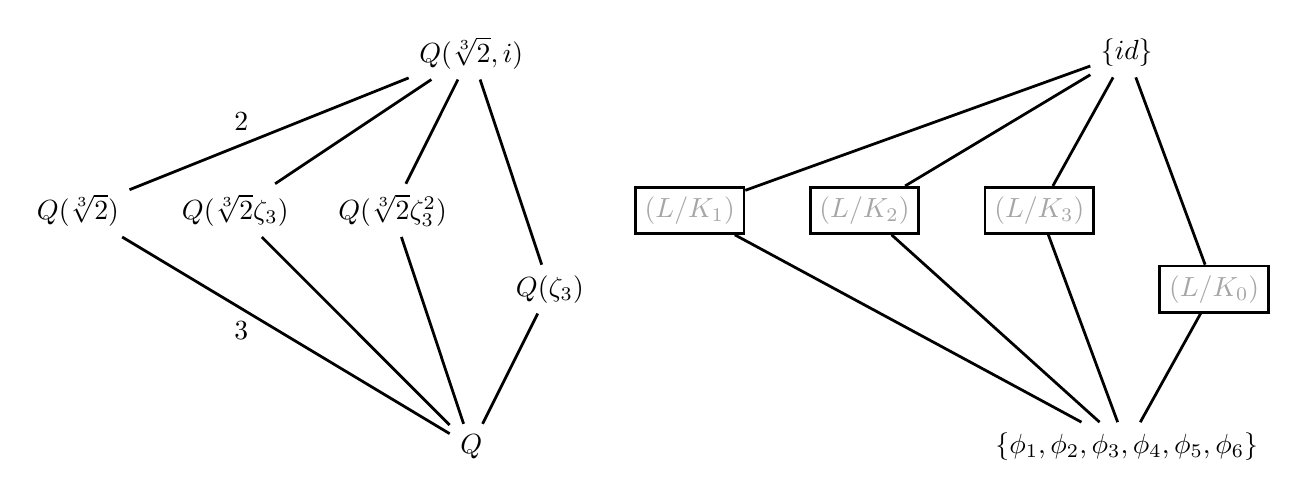
\begin{tikzpicture}[line width = 1, xscale = 1.11]
\begin{scope}[xscale = 0.9]
\node (L) at (0,4) {$\mathbb{Q}(\sqrt[3]{2},i)$}; 
\node (K1) at (-5,2) {$\mathbb{Q}(\sqrt[3]{2})$}; 
\node (K2) at (-3,2) {$\mathbb{Q}(\sqrt[3]{2}\zeta_3)$}; 
\node (K3) at (-1,2) {$\mathbb{Q}(\sqrt[3]{2}\zeta_3^2)$}; 
\node (K0) at (1,1) {$\mathbb{Q}(\zeta_3)$}; 
\node (F) at (0,-1) {$\mathbb{Q}$};

\foreach \i in {0,1,2,3} {\draw (F) -- (K\i);}
\foreach \i in {0,1,2,3} {\draw (L) -- (K\i);}

\node[anchor = 45] at (-2.7,0.7) {$3$};
\node[anchor = -45] at (-2.7,2.9) {$2$};

%\draw[line width = 0.8, ->] (1.5,4) -- (5.5,4);
%\draw[line width = 0.8, ->] (3,2) -- (4,2);
%\draw[line width = 0.8, ->] (1.5,0) -- (5.5,0);
\end{scope}

\begin{scope}[shift = {(7.5,0)}]
\node (L) at (0,4) {$\{\text{id}\}$}; 
\node[draw] (K1) at (-5,2) {\textcolor{black!35}{$\Aut(L/K_1)$}}; 
\node[draw] (K2) at (-3,2) {\textcolor{black!35}{$\Aut(L/K_2)$}};
\node[draw] (K3) at (-1,2) {\textcolor{black!35}{$\Aut(L/K_3)$}};
\node[draw] (K0) at (1,1) {\textcolor{black!35}{$\Aut(L/K_0)$}}; 
\node (F) at (0,-1) {$\{\phi_1, \phi_2,\phi_3,\phi_4,\phi_5,\phi_6\}$};

\foreach \i in {0,1,2,3} {\draw (F) -- (K\i);}
\foreach \i in {0,1,2,3} {\draw (L) -- (K\i);}
\end{scope}

\end{tikzpicture}
\end{center}
\begin{enumerate}[resume]
\item What familiar group is $\Aut(L/\mathbb{Q})$ isomorphic to?
\end{enumerate}
\end{problem}

\begin{problem}
Use Fact~\ref{fact.SizeGaloisGroup} and Problem~\ref{prob.AutQAdjoinCubeRoot2OverQ} to argue that  $\mathbb{Q}(\sqrt[3]{2})$ is \emph{not} a Galois extension of $\mathbb{Q}$ 
\end{problem}

% % % % % % % % % % % % % % % % % % % % % % % % % % % % % % % % % % % % % % % % % % % %
% SUBSECTION
% % % % % % % % % % % % % % % % % % % % % % % % % % % % % % % % % % % % % % % % % % % %
\subsection{Galois groups as permutation groups}
We now explore how to look at Galois groups as groups of permutations. The key, yet again, is Theorem~\ref{thm.HomFixingFPermutesRootsOfPolysOverF}. We begin by recalling a some definitions from group theory.

\begin{definition}
Let $X$ be a set. A bijection from $X$ to $X$ is called a \textbf{permutation} of $X$. The set of all permutations of $X$ is denoted $\operatorname{Sym}(X)$. 
The set of all permutations of $\{1,\ldots,n\}$ is usually denoted by $S_n$ (instead of $\operatorname{Sym}(\{1,\ldots,n\})$.
\end{definition}

Recall that, for any set $X$, $\operatorname{Sym}(X)$ is a group with respect to function composition. The identity is the identity function, denoted id.

\begin{theorem}\label{thm.GaloisGroupIsPermGroup}
Let $F$ be a subfield of $\mathbb{C}$. Let $p(x)\in F(x)$ be a polynomial of degree $n$, and let $R=\{r_1,\ldots,r_n\}$ be the set of all of roots of $p(x)$ in $\mathbb{C}$. Then 
\begin{enumerate} 
\item for all $\phi \in \Aut(F^{p(x)}/F)$, restricting the domain of $\phi$ to $R$ yields a permutation of $R$;
\item the map  $\Aut(F^{p(x)}/F)\to \operatorname{Sym}(R)$ that restricts the domain of each automorphism to $R$ is an injective homomorphism. 
\end{enumerate}
Consequently, $\Aut(F^{p(x)}/F)$ is isomorphic to a subgroup of $\operatorname{Sym}(R)$.
\end{theorem}

\begin{corollary}\label{cor.GaloisGroupIsPermGroup}
Let $F$ be a subfield of $\mathbb{C}$. Let $p(x)\in F(x)$ be a polynomial of degree $n$. Then $\Aut(F^{p(x)}/F)$ is isomorphic to a subgroup of $S_n$.
\end{corollary}

To view $\Aut(F^{p(x)}/F)$ as a subgroup of $S_n$, we just need to label the roots of $p(x)$ by $1,\ldots,n$ in some way and then record how each element of $\Aut(F^{p(x)}/F)$ permutes the roots. Let's take a look at an example of this.

\begin{example}\label{exam.QAdjoinZeta5GaloisAsPerms}
Similar to Problem~\ref{prob.QAdjoinZeta5IsGalois}, we can see that $\mathbb{Q}(\zeta_5) = \mathbb{Q}^{p(x)}$ for $p(x) = x^4+x^3+x^2+x+1$. We know that the set of roots of $p(x)$ is $R=\{\zeta_5,\zeta_5^2,\zeta_5^3,\zeta_5^4\}$. 

By Corollary~\ref{cor.GaloisGroupIsPermGroup}, $\Aut(\mathbb{Q}(\zeta_5)/\mathbb{Q})$ is isomorphic to a subgroup of $S_4$ because $p(x)$ has degree 4 (hence 4 roots to permute). Let's find an explicit isomorphism. Recall from Example~\ref{exam.AutQAdjoinZeta5OverQ} that the elements of $\Aut(\mathbb{Q}(\zeta_5)/\mathbb{Q})$ are defined by the following table.
\begin{center}
\tabulinesep = 2mm
\begin{tabu} spread 1in {X[$c,m]|[2pt]X[$c,m]|X[$c,m]|X[$c,m]|X[$c,m]}
 & \phi_1 & \phi_2 & \phi_3 & \phi_4  \\ \tabucline[2pt]{-}
\zeta_5 \; \mapsto  & \zeta_5 & \zeta_5^2  & \zeta_5^3  & \zeta_5^4  
\end{tabu}
\end{center}
Now let's expand the table to see how the automorphisms operate on all  roots of $p(x)$.
\begin{center}
\tabulinesep = 2mm
\begin{tabu} spread 1in {X[$c,m]|[2pt]X[$c,m]|X[$c,m]|X[$c,m]|X[$c,m]}
 & \phi_1 & \phi_2 & \phi_3 & \phi_4  \\ \tabucline[2pt]{-}
\zeta_5 \; \mapsto  & \zeta_5 & \zeta_5^2  & \zeta_5^3  & \zeta_5^4  \\ \hline
\zeta_5^2 \; \mapsto  & \zeta_5^2 & \zeta_5^4  & \zeta_5  & \zeta_5^3  \\ \hline
\zeta_5^3 \; \mapsto  & \zeta_5^3 & \zeta_5  & \zeta_5^4  & \zeta_5^2  \\ \hline
\zeta_5^4 \; \mapsto  & \zeta_5^4 & \zeta_5^3  & \zeta_5^2  & \zeta_5 
\end{tabu}
\end{center}
Next, let's identify the roots with the numbers $1$ up to $4$ as follows.
\[\zeta_5 \leftrightarrow 1\quad \zeta_5^2 \leftrightarrow 2 \quad \zeta_5^3 \leftrightarrow 3 \quad \zeta_5^4 \leftrightarrow 4.\]
%\begin{center}
%\begin{tikzpicture}[line width = 0.8, yscale = 0.8]
%\foreach \i in {1,2} {
%\node (z\i) at (0,{4-\i}) {$\zeta_5^{\i}$};
%\node (\i) at (2,{4-\i}) {$\i$};
%}
%\foreach \i in {3,4} {
%\node (z\i) at (4,{6-\i}) {$\zeta_5^{\i}$};
%\node (\i) at (6,{6-\i}) {$\i$};
%}
%\foreach \i in {1,2,3,4} {\draw[<->] (z\i) -- (\i);}
%\end{tikzpicture}
%\end{center}
Then the previous table becomes as follows.
\begin{center}
\tabulinesep = 2mm
\begin{tabu} spread 1in {X[$c,m]|[2pt]X[$c,m]|X[$c,m]|X[$c,m]|X[$c,m]}
 & \phi_1 & \phi_2 & \phi_3 & \phi_4  \\ \tabucline[2pt]{-}
1 \; \mapsto  & 1 & 2  & 3  & 4  \\ \hline
2 \; \mapsto  & 2 & 4  & 1  & 3  \\ \hline
3 \; \mapsto  & 3 & 1  & 4  & 2  \\ \hline
4 \; \mapsto  & 4 & 3  & 2  & 1
\end{tabu}
\end{center}
So, using our labeling of the four roots, we can view $\Aut(\mathbb{Q}(\zeta_5)/\mathbb{Q})$ as a subgroup of $S_4$. If we write the permutation using cycle notation, we have 
\[\phi_1 = \text{id} \quad \phi_2 = (1243) \quad \phi_2 = (1342) \quad \phi_4 = (14)(23).\]
\end{example}

\begin{problem}
Let's look at Problem~\ref{prob.AutQAdjoinSqrt2AndiOverQ} again. Notice that $\mathbb{Q}(\sqrt{2},i) = \mathbb{Q}^{p(x)}$ for $p(x) = (x^2-2)(x^2+1)$, and the set of roots of $p(x)$ are $R=\{\sqrt{2},-\sqrt{2},i,-i\}$. 
\begin{enumerate}
\item Fill in the extended table below to list how the elements of $\Aut(\mathbb{Q}(\sqrt{2},i)/\mathbb{Q})$ operate on the elements of $R$. Two of the lines were completed for you.
\begin{center}
\tabulinesep = 2mm
\begin{tabu} spread 1in {X[$r,m]|[2pt]X[$c,m]|X[$c,m]|X[$c,m]|X[$c,m]}
 & \phi_1 & \phi_2 & \phi_3 & \phi_4  \\ \tabucline[2pt]{-}
\sqrt{2} \; \mapsto\;  & \sqrt{2} &  \sqrt{2}& -\sqrt{2} &  -\sqrt{2}\\  \hline
-\sqrt{2} \; \mapsto\;  &  &  &  &   \\  \hline
i \; \mapsto \; & i & -i & i&    -i\\  \hline
-i \; \mapsto \; & &  &  &   
\end{tabu}
\end{center}
\item Label the roots of $p(x)$ via: $\sqrt{2} \leftrightarrow 1$, $-\sqrt{2}  \leftrightarrow 2$, $i \leftrightarrow 3$, and $-i \leftrightarrow 4$. Write each element of $\Aut(\mathbb{Q}(\sqrt{2},i)/\mathbb{Q})$ as a permutation in $S_4$ using cycle notation as in Example~\ref{exam.QAdjoinZeta5GaloisAsPerms}.
\end{enumerate}
\end{problem}

\begin{problem}
Let's revisit Problem~\ref{prob.AutQAdjoinCubeRoot2AndZeta3OverQ}. Set $L = \mathbb{Q}(\sqrt[3]{2},\zeta_3)$. We've seen that $L = \mathbb{Q}^{p(x)}$ for $p(x) = x^3-1$,  and the set of roots of $p(x)$ are $R=\{\sqrt[3]{2},\sqrt[3]{2}\zeta_3,\sqrt[3]{2}\zeta_3^2\}$. 
\begin{enumerate}
\item Fill in the extended table below to list how the elements of $\Aut(L/\mathbb{Q})$ operate on the elements of $R$. For the first two lines, use what you wrote in Problem~\ref{prob.AutQAdjoinCubeRoot2AndZeta3OverQ}.
\begin{center}
\tabulinesep = 2mm
\begin{tabu} spread 1in {X[$r,m]|[2pt]X[$c,m]|X[$c,m]|X[$c,m]|X[$c,m]|X[$c,m]|X[$c,m]}
 & \phi_1 & \phi_2 & \phi_3 & \phi_4  & \phi_5 & \phi_6\\ \tabucline[2pt]{-}
\sqrt[3]{2} \; \mapsto\;  & \sqrt[3]{2} &  &  & & &\\  \hline
\zeta_3 \; \mapsto \; & \zeta_3 &  &  &  & & \\ \hline
\sqrt[3]{2} \zeta_3 \; \mapsto \; &  &  &  &  & & \\ \hline
\sqrt[3]{2} \zeta_3^2 \; \mapsto \; &  &  &  &  & & \\ 
\end{tabu}
\end{center}
\item Label the elements of $R$ as follows: $\sqrt[3]{2} \leftrightarrow 1$, $\sqrt[3]{2}\zeta_3 \leftrightarrow 2$, and $\sqrt[3]{2}\zeta_3^2 \leftrightarrow 3$. Write each element of $\Aut(L/\mathbb{Q})$ as a permutation in $S_3$ using cycle notation as in Example~\ref{exam.QAdjoinZeta5GaloisAsPerms}.
\end{enumerate}
\end{problem}


